\documentclass[10pt,a4paper]{article}
\usepackage[latin1]{inputenc}
\usepackage{graphicx}
\usepackage[labelsep=quad,indention=10pt]{subfig}
\captionsetup*[subfigure]{position=bottom}
\begin{document}
    \begin{figure}[h]
        \centering
           \subfloat[edeka\_red\_bowl]{%
              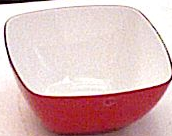
\includegraphics[height=5cm, width=4.5cm]{Bilder/edeka_red_bowl.png}%
              \label{fig:left}%
           } 
           \qquad
           \subfloat[sigg\_bottle]{%
              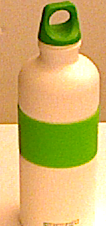
\includegraphics[height=6cm, width=3cm]{Bilder/sigg_bottle.png}%
              \label{fig:middle}%
           }
           \qquad
           \subfloat[cup\_eco\_orange]{%
              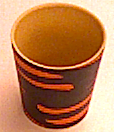
\includegraphics[height=5cm, width=3cm]{Bilder/cup_eco_orange.png}%
              \label{fig:right}%
           }
           \caption{Alle Objekte der Klasse Geschirr}
           \label{fig:default}
    \end{figure}   
    
    \begin{figure}[h]
        \centering
           \subfloat[koelln\_muesli\_knusper\_honig\_nuss]{%
              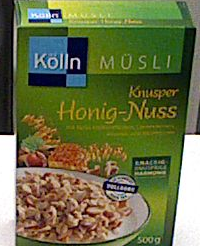
\includegraphics[height=5cm, width=4cm]{Bilder/koelln_muesli_knusper_honig_nuss.png}%
              \label{fig:left}%
           } 
           \qquad
           \subfloat[ja\_milch]{%
              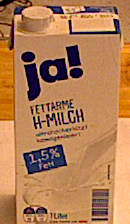
\includegraphics[height=6cm, width=3cm]{Bilder/ja_milch.png}%
              \label{fig:middle}%
           }
           \qquad
           \subfloat[kelloggs\_toppas\_mini]{%
              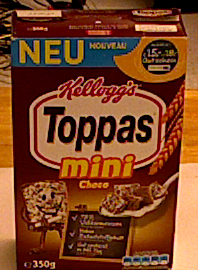
\includegraphics[height=5cm, width=3.5cm]{Bilder/kelloggs_toppas_mini.png}%
              \label{fig:right}%
           }
           \caption{Alle Objekte der Klasse Fr\"uhst\"uck}
           \label{fig:default}
    \end{figure}    
    
    \begin{figure}[h]
        \centering
           \subfloat[pringles\_paprika]{%
              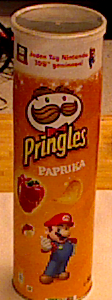
\includegraphics[height=8cm, width=3cm]{Bilder/pringles_paprika.png}%
              \label{fig:left}%
           } 
           \qquad
           \subfloat[pringles\_salt]{%
              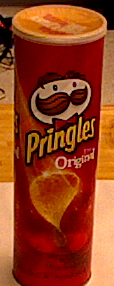
\includegraphics[height=8cm, width=3cm]{Bilder/pringles_salt.png}%
              \label{fig:middle}%
           }
           \caption{Alle Objekte der Klasse Snacks}
           \label{fig:default}
    \end{figure}    
    
    \begin{figure}[h]
        \centering
           \subfloat[tomato\_sauce\_oro\_di\_parma]{%
              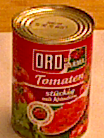
\includegraphics[height=6cm, width=4.5cm]{Bilder/tomato_sauce_oro_di_parma.png}%
              \label{fig:left}%
           } 
           \qquad
           \subfloat[hela\_curry\_ketchup]{%
              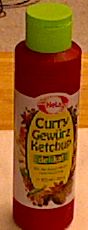
\includegraphics[height=8cm, width=3.5cm]{Bilder/hela_curry_ketchup.png}%
              \label{fig:middle}%
           }
           \caption{Alle Objekte der Klasse Saucen}
           \label{fig:default}
    \end{figure}    
\end{document}